% **************************************************************************************************************
% A Classic Thesis Style
% An Homage to The Elements of Typographic Style
%
% Copyright (C) 2011 Andr\'e Miede http://www.miede.de
%
% If you like the style then I would appreciate a postcard. My address
% can be found in the file ClassicThesis.pdf. A collection of the
% postcards I received so far is available online at
% http://postcards.miede.de
%
% License:
% This program is free software; you can redistribute it and/or modify
% it under the terms of the GNU General Public License as published by
% the Free Software Foundation; either version 2 of the License, or
% (at your option) any later version.
%
% This program is distributed in the hope that it will be useful,
% but WITHOUT ANY WARRANTY; without even the implied warranty of
% MERCHANTABILITY or FITNESS FOR A PARTICULAR PURPOSE.  See the
% GNU General Public License for more details.
%
% You should have received a copy of the GNU General Public License
% along with this program; see the file COPYING.  If not, write to
% the Free Software Foundation, Inc., 59 Temple Place - Suite 330,
% Boston, MA 02111-1307, USA.
%
% **************************************************************************************************************
% Note:
%    * You must not use "u etc. in strings/commands that will be spaced out (use \"u or real umlauts instead)
%    * New enumeration (small caps): \begin{aenumerate} \end{aenumerate}
%    * For margin notes: \graffito{}
%    * Do not use bold fonts in this style, it is designed around them
%    * Use tables as in the examples
%    * See classicthesis-ldpkg.sty for useful commands
% **************************************************************************************************************
% To Do:
%		 * [high] Check this out: http://www.golatex.de/koma-script-warnung-in-verbindung-mit-listings-package-t2058.html
%    * [medium] mathbb in section-titles/chapter-titles => disappears somehow in headlines!!!
%    * [low] Calculate text block size for Libertine font
%    * [low] Think about processing a4paper, a5paper, 10pt, 11pt, 12pt etc. options for typearea layout
%            (store values in internal variables and handle by \AtEndOfPackage{\areaset...})
% **************************************************************************************************************
\documentclass[ twoside,openright,titlepage,fleqn,numbers=noenddot,headinclude,%1headlines,% letterpaper a4paper
                11pt,a4paper,BCOR5mm,footinclude=true,cleardoublepage=empty,abstractoff % <--- obsolete, remove (todo)
                ]{scrreprt}

% ********************************************************************
% Development Stuff
% ********************************************************************
\listfiles
%\usepackage[l2tabu, orthodox, abort]{nag}
%\usepackage[warning, all]{onlyamsmath}
% ********************************************************************
% Re-usable information
% ********************************************************************
\newcommand{\myTitle}{Thesis title\xspace}
\newcommand{\myDegree}{Degree, e.g. Master Thesis / Bachelor Thesis\xspace}
\newcommand{\myName}{Name of the author\xspace}
\newcommand{\myProf}{Dr. Emanuel von Zezschwitz\xspace}
\newcommand{\myOtherProf}{Name\xspace}
\newcommand{\mySupervisor}{Name\xspace}
\newcommand{\myDepartment}{Institute of Computer Science 4\xspace}
\newcommand{\myFaculty}{Methods in Multi-Layer Usable Security Research\xspace}
\newcommand{\myUni}{\protect{Rheinische Friedrich-Wilhelms-Universit\"{a}t Bonn }\xspace}
\newcommand{\myLocation}{Bonn\xspace}
\newcommand{\myTime}{Date at which thesis is presented, e.g. March 2018\xspace}
\newcommand{\myVersion}{1.0\xspace}
%*******************************************************
% Packages with options that might require adjustments
%*******************************************************
\usepackage[latin1]{inputenc}
\usepackage[ngerman,american]{babel}
\usepackage[square,numbers]{natbib}
\usepackage{algorithm}
\usepackage{algorithmic}
\usepackage{multirow}
\usepackage{verbatim}
\usepackage[absolute]{textpos}
\usepackage{amsthm}
\newtheorem{definition}{Definition}
\usepackage[fleqn]{amsmath} % math environments and more by the AMS
%\usepackage{varioref} % load BEFORE classicthesis-ldpkg
%*******************************************************
\usepackage{classicthesis-ldpkg} % [backref]
%*******************************************************
% Options for classicthesis.sty:
% tocaligned eulerchapternumbers drafting linedheaders listings
% subfig nochapters beramono eulermath parts minionpro pdfspacing
% dottedtoc minionprospacing manychapters floatperchapter
\usepackage[eulerchapternumbers,listings,%drafting,%linedheaders,%pdfspacing,%listings,
						subfig,eulermath,parts,dottedtoc,floatperchapter]{classicthesis}%

% Change these parameters in order to resize the text area on each page
\areaset[12mm]{15cm}{761pt}%{312pt}{761pt} % Width and height of text
           \setlength{\marginparwidth}{3em}%{7em}% Width of margin
           \setlength{\marginparsep}{2em}% Distance between text and margin

%
% Use "my_enumerate" instead of "enumerate" in order to produce enumerations without vertical space between items
%
\newenvironment{my_enumerate}{
\begin{enumerate}
  \setlength{\itemsep}{1pt}
  \setlength{\parskip}{0pt}
  \setlength{\parsep}{0pt}}{\end{enumerate}
}

%*******************************************************
% Some font experiments
%*******************************************************
%\usepackage[osf]{libertine}
%\usepackage{hfoldsty}
%\usepackage[light,condensed,math]{iwona}
%\renewcommand{\sfdefault}{iwona}
%\usepackage{lmodern} % <-- no osf support :-(
%\usepackage[urw-garamond]{mathdesign} <-- no osf support :-(

%*******************************************************
% Fine-tuning for the text area
%*******************************************************
%\linespread{1.05} % a bit more for Palatino
%\areaset[5mm]{312pt}{761pt} % 686 (factor 2.2) + 33 head + 42 head \the\footskip
%\setlength{\marginparwidth}{7em}%
%\setlength{\marginparsep}{2em}%

%*******************************************************
% hack to use citations in float environments
% will be fixed with caption package version 3.2
%*******************************************************
\usepackage{makerobust}
\makeatletter
\MakeRobustCommand\caption@xref
\makeatother

%*******************************************************
%\usepackage[section,below]{placeins} <--- not everybody wants this
%\usepackage[all]{hypcap} <--- does not work with MiKTeX 2.6
% ********************************************************************
% Language/strings for backrefs (change here, thanks, Lorenzo)
%*******************************************************
%\renewcommand{\backrefnotcitedstring}{\relax}%(Not cited.)
%\renewcommand{\backrefcitedsinglestring}[1]{(Citato a pagina~#1.)}
%\renewcommand{\backrefcitedmultistring}[1]{(Citato alle pagine~#1.)}
%\renewcommand{\backreftwosep}{ e~}
%\renewcommand{\backreflastsep}{ e~}
% ********************************************************************
% Setup and Finetuning
%*******************************************************
\newlength{\abcd} % for ab..z string length calculation
\newcommand{\myfloatalign}{\centering} % how all the floats will be aligned
\setlength{\extrarowheight}{3pt} % increase table row height
% ********************************************************************
% Captions look and feel
%*******************************************************
\captionsetup{format=hang,font=small}
% ********************************************************************
% Listings setup
% ********************************************************************
%\lstset{emph={trueIndex,root},emphstyle=\color{BlueViolet}}%\underbar} % for special keywords
% ********************************************************************
\lstset{language=[LaTeX]Tex,%C++,
    keywordstyle=\color{RoyalBlue},%\bfseries,
    basicstyle=\small\ttfamily,
    %identifierstyle=\color{NavyBlue},
    commentstyle=\color{Green}\ttfamily,
    stringstyle=\rmfamily,
    numbers=none,%left,%
    numberstyle=\scriptsize,%\tiny
    stepnumber=5,
    numbersep=8pt,
    showstringspaces=false,
    breaklines=true,
    frameround=ftff,
    frame=single,
    belowcaptionskip=.75\baselineskip
    %frame=L
}

% ********************************************************************
% Where to look for graphics
%*******************************************************
%\graphicspath{{gfx/}{misc/}} % considered harmful according to l2tabu
% ********************************************************************
% Hyperreferences
%*******************************************************
\hypersetup{%
    colorlinks=true, linktocpage=true, pdfstartpage=1, pdfstartview=FitV,%
    % uncomment the following line if you want to have black links (e.g., for printing)
    %colorlinks=false, linktocpage=false, pdfborder={0 0 0}, pdfstartpage=3, pdfstartview=FitV,%
    breaklinks=true, pdfpagemode=UseNone, pageanchor=true, pdfpagemode=UseOutlines,%
    plainpages=false, bookmarksnumbered, bookmarksopen=true, bookmarksopenlevel=1,%
    hypertexnames=true, pdfhighlight=/O,%hyperfootnotes=true,%nesting=true,%frenchlinks,%
    urlcolor=webbrown, linkcolor=RoyalBlue, citecolor=webgreen, %pagecolor=RoyalBlue,%
    %urlcolor=Black, linkcolor=Black, citecolor=Black, %pagecolor=Black,%
    pdftitle={\myTitle},%
    pdfauthor={\textcopyright\ \myName, \myUni, \myFaculty},%
    pdfsubject={},%
    pdfkeywords={},%
    pdfcreator={pdfLaTeX},%
    pdfproducer={LaTeX with hyperref and classicthesis}%
}

%********************************************************************
% Hyphenation
%*******************************************************
%\hyphenation{put special hyphenation here}
% ********************************************************************
% GO!GO!GO! MOVE IT!
%*******************************************************
\begin{document}
\frenchspacing
\raggedbottom
\selectlanguage{american} % american ngerman
%\renewcommand*{\bibname}{new name}
%\setbibpreamble{}
\pagenumbering{roman}
\pagestyle{plain}
%********************************************************************
% Frontmatter
%*******************************************************
%%*******************************************************
% Little Dirty Titlepage
%*******************************************************
\thispagestyle{empty}
%\pdfbookmark[1]{Titel}{title}
%*******************************************************
\begin{center}
    \spacedlowsmallcaps{\myName} \\ \medskip                        

    \begingroup
        \color{Maroon}\spacedallcaps{\myTitle}
    \endgroup
\end{center}        

%*******************************************************
% Titlepage
%*******************************************************
\begin{titlepage}

    \begin{comment}
    \begin{textblock*}{297mm}(0mm,0mm)
        \includegraphics[width=\paperwidth]{gfx/titlePage}
    \end{textblock*}
    \phantom{Invisible, but important}
    \newpage
    \end{comment}

	% if you want the titlepage to be centered, uncomment and fine-tune the line below (KOMA classes environment)
	\begin{addmargin}[-2cm]{-2.5cm}
    \begin{center}
        \large
        
		\begin{flushleft}
		
\includegraphics[width=6cm]{gfx/logos/unilogobonn}
		\end{flushleft}
       
        \vfill

        \begingroup
            %\color{Blue}\spacedallcaps{\myTitle} \\ \bigskip
            \color{Blue}\spacedallcaps{\myTitle} \bigskip
        \endgroup

        \spacedlowsmallcaps{\myName}

        \vfill

        \medskip

        \myDegree \\ \medskip
        \myTime

        \bigskip

        \vfill

	\myUni \\
        \myDepartment \\
        \myFaculty \\
        %\myUni \\
      %  \includegraphics[width=5cm]{gfx/logos/seemoo_logo} \\

        %\vfill

    \end{center}
  \end{addmargin}
\end{titlepage}   
\thispagestyle{empty}

\noindent\myTitle \\
\noindent\myDegree \\
%\noindent UBIPS-xSC-xxxx

\bigskip

\noindent Submitted by \myName \\
\noindent Date of submission:

\bigskip

\noindent  First examiner/Erstgutachter: \myProf \\
\noindent Second examiner/Zweitgutachter: \myOtherProf \\
\noindent Supervisor/Betreuer: \mySupervisor \\

\hfill

\vfill

\noindent \myUni \\
\noindent \myDepartment \\
\noindent \myFaculty \\

%\noindent\myName: \textit{\myTitle,} \myDegree, \textcopyright\ \myTime

%\bigskip
%
%\noindent\spacedlowsmallcaps{Supervisors}: \\
%\myProf \\
%\myOtherProf \\
%\mySupervisor
%
%\medskip
%
%\noindent\spacedlowsmallcaps{Location}: \\
%\myLocation
%
%\medskip
%
%\noindent\spacedlowsmallcaps{Time Frame}: \\
%\myTime

%\cleardoublepage%*******************************************************
% Dedication
%*******************************************************
\thispagestyle{empty}
%\phantomsection 
\refstepcounter{dummy}
\pdfbookmark[1]{Dedication}{Dedication}

\vspace*{3cm}

\begin{center}
    \emph{Ohana} means family. \\
    Family means nobody gets left behind, or forgotten. \\ \medskip
    --- Lilo \& Stitch    
\end{center}

\medskip

\begin{center}
    Dedicated to the loving memory of Rudolf Miede. \\ \smallskip
    1939\,--\,2005
\end{center}
\cleardoublepage%*******************************************************
% Abstract
%*******************************************************
%\renewcommand{\abstractname}{Abstract}
\pdfbookmark[1]{Abstract}{Abstract}
\begingroup
\let\clearpage\relax
\let\cleardoublepage\relax
\let\cleardoublepage\relax

\chapter*{Abstract}
Abstract in English

\vfill

\pdfbookmark[1]{Zusammenfassung}{Zusammenfassung}
\chapter*{Zusammenfassung}
Kurze Zusammenfassung auf Deutsch


\endgroup			

\vfill 
\cleardoublepage%*******************************************************
% Declaration
%*******************************************************
\refstepcounter{dummy}
\pdfbookmark[0]{Declaration}{declaration}
\chapter*{Erkl{\"a}rung zur Master-Thesis / Bachelor-Thesis}
\thispagestyle{empty}
Hiermit versichere ich, die vorliegende Master-Thesis / Bachelor-Thesis ohne Hilfe Dritter nur mit den angegebenen Quellen und Hilfsmitteln angefertigt zu haben. Alle Stellen, die aus Quellen entnommen wurden, sind als solche kenntlich gemacht. Diese Arbeit hat in gleicher oder {\"a}hnlicher Form noch keiner Pr{\"u}fungsbeh{\"o}rde vorgelegen.
\bigskip

\noindent\textit{\myLocation, \myTime}

\smallskip

\begin{flushright}
    \begin{tabular}{m{5cm}}
        \\ \hline
        \centering\myName \\
    \end{tabular}
\end{flushright}

%\cleardoublepage%*******************************************************
% Publications
%*******************************************************
\pdfbookmark[1]{Publications}{publications}
\chapter*{Publications}
Some ideas and figures have appeared previously in the following publications:

\bigskip

\noindent Put your publications from the thesis here. The packages \texttt{multibib} or \texttt{bibtopic} etc. can be used to handle multiple different bibliographies in your document.
%\cleardoublepage%*******************************************************
% Acknowledgments
%*******************************************************
\pdfbookmark[1]{Acknowledgments}{acknowledgments}

\begin{flushright}{\slshape    
    We have seen that computer programming is an art, \\ 
    because it applies accumulated knowledge to the world, \\ 
    because it requires skill and ingenuity, and especially \\
    because it produces objects of beauty.} \\ \medskip
    --- \defcitealias{knuth:1974}{Donald E. Knuth}\citetalias{knuth:1974} \citep{knuth:1974}
\end{flushright}



\bigskip

\begingroup
\let\clearpage\relax
\let\cleardoublepage\relax
\let\cleardoublepage\relax
\chapter*{Acknowledgments}
Put your acknowledgments here.

Many thanks to everybody who already sent me a postcard!

Regarding the typography and other help, many thanks go to Marco 
Kuhlmann, Philipp Lehman, Lothar Schlesier, Jim Young, Lorenzo 
Pantieri and Enrico Gregorio\footnote{Members of GuIT (Gruppo 
Italiano Utilizzatori di \TeX\ e \LaTeX )}, J\"org Sommer, 
Joachim K\"ostler, Daniel Gottschlag, Denis Aydin, Paride 
Legovini, Steffen Prochnow, Nicolas Repp, Hinrich Harms, 
and the whole \LaTeX-community for support, ideas and some great software.

\endgroup




\pagestyle{scrheadings}
\cleardoublepage%*******************************************************
% Table of Contents
%*******************************************************
%\phantomsection
\refstepcounter{dummy}
\pdfbookmark[1]{\contentsname}{tableofcontents}
\setcounter{tocdepth}{2} % <-- 2 includes up to subsections in the ToC
\setcounter{secnumdepth}{3} % <-- 3 numbers up to subsubsections
\manualmark
\markboth{\spacedlowsmallcaps{\contentsname}}{\spacedlowsmallcaps{\contentsname}}
\tableofcontents
\automark[section]{chapter}
\renewcommand{\chaptermark}[1]{\markboth{\spacedlowsmallcaps{#1}}{\spacedlowsmallcaps{#1}}}
\renewcommand{\sectionmark}[1]{\markright{\thesection\enspace\spacedlowsmallcaps{#1}}}
%*******************************************************
% List of Figures and of the Tables
%*******************************************************
\clearpage

\begingroup
    \let\clearpage\relax
    \let\cleardoublepage\relax
    \let\cleardoublepage\relax
%    %*******************************************************
%    % List of Figures
%    %*******************************************************
%    %\phantomsection
%    \refstepcounter{dummy}
%    %\addcontentsline{toc}{chapter}{\listfigurename}
%    \pdfbookmark[1]{\listfigurename}{lof}
%    \listoffigures
%
%    \vspace*{8ex}
%
%    %*******************************************************
%    % List of Tables
%    %*******************************************************
%    %\phantomsection
%    \refstepcounter{dummy}
%    %\addcontentsline{toc}{chapter}{\listtablename}
%    \pdfbookmark[1]{\listtablename}{lot}
%    \listoftables
%
%    \vspace*{8ex}
%%   \newpage
%
%    %*******************************************************
%    % List of Algorithms
%    %*******************************************************
%	%\phantomsection
%    \refstepcounter{dummy}
%    %\addcontentsline{toc}{chapter}{\lstlistlistingname}
%    \pdfbookmark[1]{Algorithms}{lol}
%    \listofalgorithms
%
%    %\vspace*{8ex}
%
%    %*******************************************************
    % Acronyms
    %*******************************************************
    %\phantomsection
    \refstepcounter{dummy}
    \pdfbookmark[1]{Acronyms}{acronyms}
    \markboth{\spacedlowsmallcaps{Acronyms}}{\spacedlowsmallcaps{Acronyms}}
    \chapter*{Acronyms}
    \begin{acronym}[UML]
        \acro{DRY}{Don't Repeat Yourself}
        \acro{API}{Application Programming Interface}
        \acro{UML}{Unified Modeling Language}
    \end{acronym}
    
\endgroup

\cleardoublepage 
%********************************************************************
% Mainmatter
%*******************************************************
\pagenumbering{arabic}
\setcounter{page}{1}
% use \cleardoublepage here to avoid problems with pdfbookmark
%\cleardoublepage\myPart{Some Kind of Manual}
%************************************************
\chapter{First chapter}\label{ch:first}
%************************************************
This is the first chapter. For more information on this template, see the documentation of the "Classic Thesis" template by Andr� Miede \url{http://www.ctan.org/tex-archive/macros/latex/contrib/classicthesis/}. The following hints might be interesting for typesetting your thesis:

\begin{enumerate}
    \item At the beginning of the file "thesis.tex", substitute the thesis title, date, name etc. by your own
    \item It is recommendable to write each chapter in a separate TEX file
    \item At the end of the file "thesis.tex", include all external TEX files you wish to include (e.g. chapters, appendices, acknowledgements, dedications etc.)
    \item Line 95 of "thesis.tex" allows you to change the text margins of your thesis
    \item The rest of this chapter includes examples for images, tables, footnotes etc.
\end{enumerate}

Lorem ipsum dolor sit amet, consectetur adipiscing elit. Nulla consequat elementum justo a scelerisque. Nam a urna a velit pretium malesuada. Nulla facilisi. Praesent sollicitudin sodales luctus. Sed eros ipsum, auctor vitae interdum vel, varius id sem. Donec iaculis, nulla nec gravida pharetra, est purus rutrum lorem, ut pretium nulla sem eget elit. Duis eu adipiscing augue. Vestibulum et mattis magna. Curabitur sit amet est eu tortor tristique sodales. Morbi ullamcorper facilisis est ac commodo. Mauris lacinia leo et enim vehicula convallis mattis nisi venenatis. Nulla lacus lorem, tincidunt id consectetur sed, ultricies at felis. Vestibulum eu sem non est facilisis pulvinar. Suspendisse dui nibh, pulvinar tempor cursus eget, egestas id augue. Mauris molestie erat sed turpis luctus aliquet. Donec sed pellentesque purus. Integer et nunc mauris.


\section{Examples}

Within a section, you can create a subsection and a subsubsection. Moreover, you can include footnotes\footnote{This is a footnote}. Lorem ipsum dolor sit amet, consectetur adipiscing elit. Nulla consequat elementum justo a scelerisque. Nam a urna a velit pretium malesuada. Nulla facilisi. Praesent sollicitudin sodales luctus. Sed eros ipsum, auctor vitae interdum vel, varius id sem. Donec iaculis, nulla nec gravida pharetra, est purus rutrum lorem, ut pretium nulla sem eget elit. Duis eu adipiscing augue.

\subsection{Subsections}

Subsections are included in the index. Lorem ipsum dolor sit amet, consectetur adipiscing elit. Nulla consequat elementum justo a scelerisque. Nam a urna a velit pretium malesuada. Nulla facilisi. Praesent sollicitudin sodales luctus. Sed eros ipsum, auctor vitae interdum vel, varius id sem. Donec iaculis, nulla nec gravida pharetra, est purus rutrum lorem, ut pretium nulla sem eget elit. Duis eu adipiscing augue. Vestibulum et mattis magna. Curabitur sit amet est eu tortor tristique sodales.

\subsubsection{This is a subsubsection}

Subsubsections are not included in the index. Lorem ipsum dolor sit amet, consectetur adipiscing elit. Nulla consequat elementum justo a scelerisque. Nam a urna a velit pretium malesuada. Nulla facilisi. Praesent sollicitudin sodales luctus. Sed eros ipsum, auctor vitae interdum vel, varius id sem. Donec iaculis, nulla nec gravida pharetra, est purus rutrum lorem, ut pretium nulla sem eget elit. Duis eu adipiscing augue. Vestibulum et mattis magna. Curabitur sit amet est eu tortor tristique sodales. Morbi ullamcorper facilisis est ac commodo. Mauris lacinia leo et enim vehicula convallis mattis nisi venenatis. Nulla lacus lorem, tincidunt id consectetur sed, ultricies at felis. Vestibulum eu sem non est facilisis pulvinar. Suspendisse dui nibh, pulvinar tempor cursus eget, egestas id augue. Mauris molestie erat sed turpis luctus aliquet. Donec sed pellentesque purus. Integer et nunc mauris.

\subsubsection{And another subsubsection}

Lorem ipsum dolor sit amet, consectetur adipiscing elit. Nulla consequat elementum justo a scelerisque. Nam a urna a velit pretium malesuada. Nulla facilisi. Praesent sollicitudin sodales luctus. Sed eros ipsum, auctor vitae interdum vel, varius id sem. Donec iaculis, nulla nec gravida pharetra, est purus rutrum lorem, ut pretium nulla sem eget elit. Duis eu adipiscing augue. Vestibulum et mattis magna. Curabitur sit amet est eu tortor tristique sodales. Morbi ullamcorper facilisis est ac commodo. Mauris lacinia leo et enim vehicula convallis mattis nisi venenatis. Nulla lacus lorem, tincidunt id consectetur sed, ultricies at felis. Vestibulum eu sem non est facilisis pulvinar. Suspendisse dui nibh, pulvinar tempor cursus eget, egestas id augue. Mauris molestie erat sed turpis luctus aliquet. Donec sed pellentesque purus. Integer et nunc mauris.

\subsection{Images}

In this subsection we include some image examples. First, a single image in Figure~\ref{fig:single_image}, and second, multiple side-by-side images in Figure~\ref{fig:side_by_side}. Images can be in JPG and PDF format.

\begin{figure}[h]
\centering
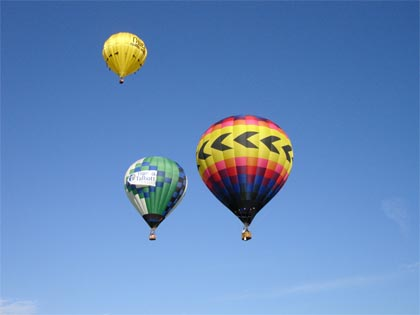
\includegraphics[width=10cm]{gfx/sample1}
\caption[This is a short caption for the index]{This is a long caption, which will be placed below the image}
\label{fig:single_image}
\end{figure}

Lorem ipsum dolor sit amet, consectetur adipiscing elit. Nulla consequat elementum justo a scelerisque. Nam a urna a velit pretium malesuada. Nulla facilisi. Praesent sollicitudin sodales luctus. Sed eros ipsum, auctor vitae interdum vel, varius id sem. Donec iaculis, nulla nec gravida pharetra, est purus rutrum lorem, ut pretium nulla sem eget elit. Duis eu adipiscing augue.

\begin{figure}[h!]
    \myfloatalign
    \subfloat[Caption of image 1]
    {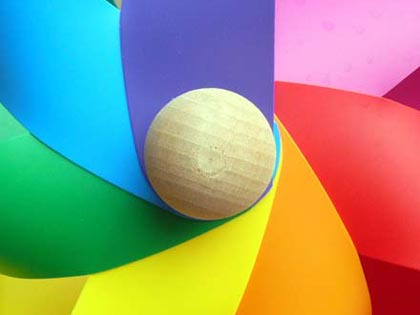
\includegraphics[width=.35\linewidth]{gfx/sample2}} \quad
    \subfloat[Caption of image 2]
    {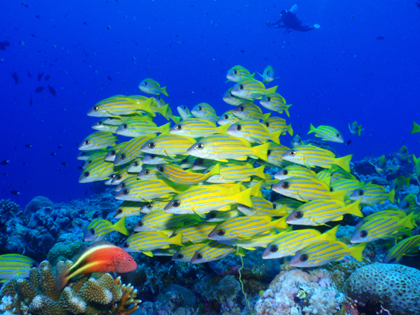
\includegraphics[width=.35\linewidth]{gfx/sample3}} \\
    \subfloat[Caption of image 3]
    {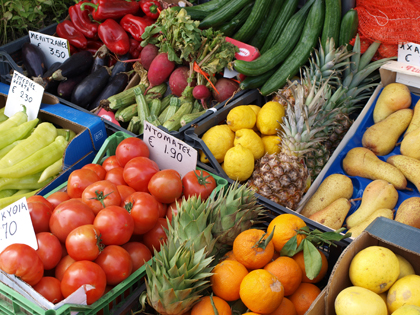
\includegraphics[width=.35\linewidth]{gfx/sample4}} \quad
    \subfloat[Caption of image 4]
    {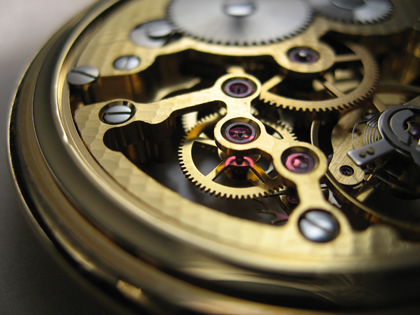
\includegraphics[width=.35\linewidth]{gfx/sample5}} \\
    \subfloat[Caption of image 5]
    {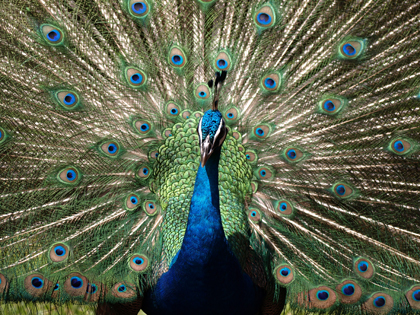
\includegraphics[width=.35\linewidth]{gfx/sample6}} \quad
    \subfloat[Caption of image 6]
    {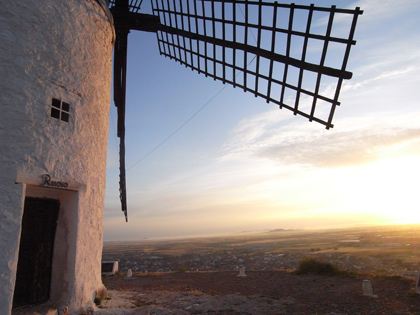
\includegraphics[width=.35\linewidth]{gfx/sample7}}
    \caption[Side-by-side image]{Caption for all images.}
    \label{fig:side_by_side}
\end{figure}


\subsection{Tables}

See Table~\ref{tab:example}. Lorem ipsum dolor sit amet, consectetur adipiscing elit. Nulla consequat elementum justo a scelerisque. Nam a urna a velit pretium malesuada. Nulla facilisi. Praesent sollicitudin sodales luctus. Sed eros ipsum, auctor vitae interdum vel, varius id sem. Donec iaculis, nulla nec gravida pharetra, est purus rutrum lorem, ut pretium nulla sem eget elit. Duis eu adipiscing augue. Vestibulum et mattis magna.

\begin{table}
    \myfloatalign
  \begin{tabularx}{15cm}{p{1cm} p{3cm} p{8.5cm}}
    \toprule
    \tableheadline{Test} & \tableheadline{Test} & \tableheadline{Test} \\ \midrule
    Test & Example &  Lorem ipsum dolor sit amet, consectetur adipiscing elit. Nulla consequat elementum justo a scelerisque. Nam a urna a velit pretium malesuada. \\
    \midrule
    Test & Example &  Lorem ipsum dolor sit amet, consectetur adipiscing elit. Nulla consequat elementum justo a scelerisque. Nam a urna a velit pretium malesuada. \\
    \midrule
    Test & Example &  Lorem ipsum dolor sit amet, consectetur adipiscing elit. Nulla consequat elementum justo a scelerisque. Nam a urna a velit pretium malesuada. \\
    \midrule
    Test & Example &  Lorem ipsum dolor sit amet, consectetur adipiscing elit. Nulla consequat elementum justo a scelerisque. Nam a urna a velit pretium malesuada. \\
    \bottomrule
  \end{tabularx}
  \caption[Table example]{Table example}
  \label{tab:example}
\end{table}

\subsection{Citations}

You can cite the items listed in the "Bibliography.bib" file, like for example \cite{bentley:1999} and \cite{bringhurst:2002}. However, in the sample bibliography, there are more publications, like \cite{cormen:2001}, \cite{dueck:trio} and \cite{knuth:1974}. Lorem ipsum dolor sit amet, consectetur adipiscing elit. Nulla consequat elementum justo a scelerisque. Nam a urna a velit pretium malesuada. Nulla facilisi. Praesent sollicitudin sodales luctus. Sed eros ipsum, auctor vitae interdum vel, varius id sem. Donec iaculis, nulla nec gravida pharetra, est purus rutrum lorem, ut pretium nulla sem eget elit. Duis eu adipiscing augue. Vestibulum et mattis magna.

\subsection{References}

We include a sample second chapter and an appendix. However, neither Chapter~\ref{ch:second} nor Appendix~\ref{ch:appendix} are actually interesting, since they only contain more Lorem ipsum. Lorem ipsum dolor sit amet, consectetur adipiscing elit. Nulla consequat elementum justo a scelerisque. Nam a urna a velit pretium malesuada. Nulla facilisi. Praesent sollicitudin sodales luctus. Sed eros ipsum, auctor vitae interdum vel, varius id sem. Donec iaculis, nulla nec gravida pharetra, est purus rutrum lorem, ut pretium nulla sem eget elit. Duis eu adipiscing augue. Vestibulum et mattis magna. Curabitur sit amet est eu tortor tristique sodales. Morbi ullamcorper facilisis est ac commodo. Mauris lacinia leo et enim vehicula convallis mattis nisi venenatis.

\section{Another section}

Lorem ipsum dolor sit amet, consectetur adipiscing elit. Morbi lorem ipsum, posuere vitae mattis sed, dictum in leo. Aenean felis diam, egestas a tincidunt id, tincidunt aliquam dui. Fusce posuere sagittis ipsum, eu tristique ligula elementum vitae. Aliquam erat volutpat. Donec sed erat lobortis nisl hendrerit pretium. Integer at bibendum est. Sed dapibus quam ut dui sodales auctor. Donec sodales orci condimentum erat euismod viverra. Aliquam ullamcorper ligula ac velit cursus fermentum. Pellentesque laoreet, libero eu rutrum dapibus, tellus velit tristique massa, id dignissim urna erat semper ligula.

Cras et venenatis nibh. Vestibulum hendrerit egestas lorem vitae congue. Vivamus vitae vehicula lacus. Nam pellentesque tellus eget massa aliquam nec lacinia tellus porta. Curabitur consectetur ligula ut felis convallis elementum vitae vel nibh. Maecenas id felis lectus, ac scelerisque arcu. Morbi ut pharetra neque. Curabitur sit amet eros in justo aliquam rutrum. Nullam sed rutrum massa. Vestibulum consequat sem interdum justo fringilla ac condimentum odio ullamcorper. Nam fermentum nibh nisi, ut consectetur dui. Nunc fringilla congue ligula eu congue.

Integer dignissim porta nulla, sed sollicitudin nisl placerat pulvinar. Aliquam placerat tincidunt urna, volutpat tristique neque eleifend quis. Curabitur luctus erat vitae odio posuere a bibendum neque adipiscing. Aliquam malesuada lectus tortor. In malesuada mi et dui molestie viverra placerat nibh aliquam. Praesent nunc risus, rhoncus posuere iaculis vel, molestie ut mauris. Quisque faucibus, mauris eu congue pretium, eros turpis pharetra nisl, quis luctus massa dolor et est. Donec eu odio in elit tincidunt mollis. Integer eleifend ullamcorper sem ac tristique. Aliquam consequat lorem vitae dolor egestas pharetra sagittis urna volutpat. Nullam adipiscing urna tellus, vitae vestibulum mauris. In hac habitasse platea dictumst. Cras ipsum lorem, ultricies eu pretium vel, feugiat sed tortor. Nunc consectetur, urna ut porttitor lobortis, nulla quam mattis tellus, id egestas massa diam eu enim. Quisque eget urna risus. Mauris nec lorem quis felis fringilla porta. Phasellus porttitor, nisi in consequat blandit, massa turpis volutpat sem, eget condimentum felis leo in erat. Sed et est mauris. 
%*****************************************
\chapter{Second chapter}\label{ch:second}
%*****************************************
Lorem ipsum dolor sit amet, consectetur adipiscing elit. Maecenas faucibus adipiscing magna at pellentesque. Donec nibh turpis, cursus a sollicitudin commodo, imperdiet vulputate nibh. Donec mattis erat sit amet lectus ultricies lobortis. Morbi aliquam diam sit amet augue faucibus eget vehicula tortor egestas. Nulla in mi in tortor gravida gravida. Aenean tempus nisi vel magna volutpat ullamcorper. Etiam semper ultrices suscipit. Quisque varius erat ac lorem sodales interdum. Vivamus pharetra imperdiet orci, ut malesuada mi fermentum ut. Pellentesque eget venenatis mi. Proin condimentum augue a metus suscipit et porttitor justo egestas. Aliquam erat volutpat. Aliquam pretium massa et elit fringilla egestas. Aliquam varius mi at eros lobortis ac consectetur nisl blandit. In hac habitasse platea dictumst. Maecenas nisl odio, cursus accumsan ultricies in, dignissim sed arcu. Aenean nisi lorem, ornare sed sodales vel, faucibus quis sapien. Suspendisse lorem arcu, dapibus tempor luctus nec, vestibulum a est.

Nulla feugiat dui elementum ante pharetra sit amet tempus quam viverra. Cras odio urna, tempor ac aliquam in, laoreet in mi. Vivamus commodo rhoncus erat, in venenatis dolor gravida id. Duis consectetur pretium scelerisque. Quisque dapibus sodales adipiscing. Suspendisse potenti. Nulla neque leo, fermentum non luctus sit amet, vulputate id quam. Nam vel mi id dui aliquet sodales et at dui. Cras vel mauris arcu. Praesent scelerisque massa at justo vehicula non tristique neque consequat. Curabitur in posuere elit. Vestibulum euismod volutpat ligula, a blandit sapien ornare ac. Nulla placerat tempor tempus. Praesent cursus dui malesuada nibh venenatis vel varius augue fringilla.

Quisque blandit lobortis nibh nec elementum. Lorem ipsum dolor sit amet, consectetur adipiscing elit. Quisque hendrerit auctor dignissim. Duis a placerat nibh. Phasellus in eros augue, in condimentum nisl. Curabitur dapibus varius sollicitudin. Nam lobortis egestas nibh, quis condimentum massa faucibus non. Suspendisse hendrerit varius accumsan. Cum sociis natoque penatibus et magnis dis parturient montes, nascetur ridiculus mus. Nunc nisi erat, ultricies eget fringilla vel, ullamcorper et dui. Curabitur vel justo neque, sit amet mollis arcu. Phasellus eleifend fringilla tellus quis egestas. Praesent non enim sit amet erat suscipit vulputate. Morbi in fermentum metus. Sed orci risus, iaculis nec dapibus nec, rutrum in magna. Curabitur at orci sed nisi ornare tincidunt eu non augue.

Pellentesque in arcu turpis. Nulla fermentum justo eget urna elementum sit amet imperdiet nibh posuere. Nullam at vehicula erat. Ut feugiat sollicitudin blandit. Fusce adipiscing pulvinar interdum. Donec non nisi arcu. Sed et leo at neque imperdiet placerat sed sit amet dui. Aenean vitae nisi tellus. Sed erat erat, molestie a pulvinar at, imperdiet in lacus. Nullam facilisis nibh vel augue tristique volutpat. Quisque lorem est, luctus et egestas in, ultricies ut eros. In venenatis felis nec massa accumsan et pellentesque lacus vulputate. Fusce scelerisque augue vehicula est commodo fermentum. Pellentesque quis turpis magna. Aliquam erat volutpat. Curabitur eget augue et sapien accumsan ultrices nec ac sem. Aliquam gravida orci at dui lacinia tincidunt. Donec tristique ipsum faucibus orci auctor venenatis. Suspendisse condimentum, magna mattis adipiscing tempor, mi nisl dictum ante, vitae sodales magna urna quis enim. Nulla eu nibh turpis, id bibendum leo.

Sed semper sem in dui mattis tristique. Proin auctor nunc quis nibh congue iaculis. Ut at nisl a massa lobortis pretium eu eget justo. Morbi eu elit quis tellus dictum ornare. Ut tempus purus a lectus varius a vestibulum nibh venenatis. Donec dapibus facilisis tellus, tincidunt tempus metus congue a. In quis vulputate felis. Maecenas a sapien tellus. Suspendisse ut tellus est. Nunc risus elit, eleifend ullamcorper scelerisque ac, sodales sed sem.

Donec et nibh dignissim nisi vehicula consectetur. Praesent et arcu massa. Maecenas congue lacinia lacinia. Nullam scelerisque molestie aliquam. Maecenas lacus diam, pretium in convallis ut, suscipit eu mi. Phasellus eu sodales metus. Aliquam ut urna lectus, nec congue mauris. Suspendisse vel dignissim risus. Phasellus risus odio, sodales sed pretium ac, pulvinar vel magna. Integer urna leo, dapibus vitae porta nec, sollicitudin quis neque. Quisque urna magna, ultricies at venenatis vitae, scelerisque eget mauris. Class aptent taciti sociosqu ad litora torquent per conubia nostra, per inceptos himenaeos. Suspendisse at est est. Fusce vel suscipit ipsum. Phasellus felis sem, commodo posuere fermentum vitae, gravida eget eros. Nunc nulla felis, fringilla id vehicula ut, rhoncus non ligula. Etiam pulvinar aliquam lorem, a congue dolor malesuada eu. Duis vulputate tellus nec nunc dignissim nec scelerisque massa placerat.

Vestibulum convallis, quam sit amet congue feugiat, risus odio vulputate dui, ac bibendum lacus ligula nec tortor. Curabitur non urna ipsum. Nullam pulvinar rhoncus lectus, nec sollicitudin felis pharetra ut. Donec lacinia, leo quis interdum tincidunt, justo mi tristique enim, quis ultrices sapien magna vel odio. Mauris volutpat vulputate purus, non dictum tellus consectetur id. In et felis ac tortor luctus pharetra in sed odio. Proin pulvinar tempus quam in porta. Aliquam nibh nibh, vehicula sit amet luctus ac, consectetur ac eros. Pellentesque habitant morbi tristique senectus et netus et malesuada fames ac turpis egestas. Maecenas eget elit ac orci vestibulum tristique vitae id ante. Cras et felis ac neque pharetra adipiscing. Mauris rhoncus, lacus at euismod eleifend, turpis leo molestie arcu, a rhoncus sem ante volutpat nunc. Suspendisse id viverra diam. Fusce semper arcu nisl.
%\addtocontents{toc}{\protect\clearpage} % <--- just debug stuff, ignore
%\include{Chapters/Chapter03}
%\include{multiToC} % <--- just debug stuff, ignore for your documents
% ********************************************************************
% Backmatter
%*******************************************************
\appendix
%\cleardoublepage\part{Appendix}
%*******************************************************
% Appendix - CBF algorithm
%*******************************************************
\chapter{Appendix}\label{ch:appendix}
Lorem ipsum dolor sit amet, consectetur adipiscing elit. Maecenas faucibus adipiscing magna at pellentesque. Donec nibh turpis, cursus a sollicitudin commodo, imperdiet vulputate nibh. Donec mattis erat sit amet lectus ultricies lobortis. Morbi aliquam diam sit amet augue faucibus eget vehicula tortor egestas. Nulla in mi in tortor gravida gravida. Aenean tempus nisi vel magna volutpat ullamcorper. Etiam semper ultrices suscipit. Quisque varius erat ac lorem sodales interdum. Vivamus pharetra imperdiet orci, ut malesuada mi fermentum ut. Pellentesque eget venenatis mi. Proin condimentum augue a metus suscipit et porttitor justo egestas. Aliquam erat volutpat. Aliquam pretium massa et elit fringilla egestas. Aliquam varius mi at eros lobortis ac consectetur nisl blandit. In hac habitasse platea dictumst. Maecenas nisl odio, cursus accumsan ultricies in, dignissim sed arcu. Aenean nisi lorem, ornare sed sodales vel, faucibus quis sapien. Suspendisse lorem arcu, dapibus tempor luctus nec, vestibulum a est.

Nulla feugiat dui elementum ante pharetra sit amet tempus quam viverra. Cras odio urna, tempor ac aliquam in, laoreet in mi. Vivamus commodo rhoncus erat, in venenatis dolor gravida id. Duis consectetur pretium scelerisque. Quisque dapibus sodales adipiscing. Suspendisse potenti. Nulla neque leo, fermentum non luctus sit amet, vulputate id quam. Nam vel mi id dui aliquet sodales et at dui. Cras vel mauris arcu. Praesent scelerisque massa at justo vehicula non tristique neque consequat. Curabitur in posuere elit. Vestibulum euismod volutpat ligula, a blandit sapien ornare ac. Nulla placerat tempor tempus. Praesent cursus dui malesuada nibh venenatis vel varius augue fringilla.

Quisque blandit lobortis nibh nec elementum. Lorem ipsum dolor sit amet, consectetur adipiscing elit. Quisque hendrerit auctor dignissim. Duis a placerat nibh. Phasellus in eros augue, in condimentum nisl. Curabitur dapibus varius sollicitudin. Nam lobortis egestas nibh, quis condimentum massa faucibus non. Suspendisse hendrerit varius accumsan. Cum sociis natoque penatibus et magnis dis parturient montes, nascetur ridiculus mus. Nunc nisi erat, ultricies eget fringilla vel, ullamcorper et dui. Curabitur vel justo neque, sit amet mollis arcu. Phasellus eleifend fringilla tellus quis egestas. Praesent non enim sit amet erat suscipit vulputate. Morbi in fermentum metus. Sed orci risus, iaculis nec dapibus nec, rutrum in magna. Curabitur at orci sed nisi ornare tincidunt eu non augue.

Pellentesque in arcu turpis. Nulla fermentum justo eget urna elementum sit amet imperdiet nibh posuere. Nullam at vehicula erat. Ut feugiat sollicitudin blandit. Fusce adipiscing pulvinar interdum. Donec non nisi arcu. Sed et leo at neque imperdiet placerat sed sit amet dui. Aenean vitae nisi tellus. Sed erat erat, molestie a pulvinar at, imperdiet in lacus. Nullam facilisis nibh vel augue tristique volutpat. Quisque lorem est, luctus et egestas in, ultricies ut eros. In venenatis felis nec massa accumsan et pellentesque lacus vulputate. Fusce scelerisque augue vehicula est commodo fermentum. Pellentesque quis turpis magna. Aliquam erat volutpat. Curabitur eget augue et sapien accumsan ultrices nec ac sem. Aliquam gravida orci at dui lacinia tincidunt. Donec tristique ipsum faucibus orci auctor venenatis. Suspendisse condimentum, magna mattis adipiscing tempor, mi nisl dictum ante, vitae sodales magna urna quis enim. Nulla eu nibh turpis, id bibendum leo.

Sed semper sem in dui mattis tristique. Proin auctor nunc quis nibh congue iaculis. Ut at nisl a massa lobortis pretium eu eget justo. Morbi eu elit quis tellus dictum ornare. Ut tempus purus a lectus varius a vestibulum nibh venenatis. Donec dapibus facilisis tellus, tincidunt tempus metus congue a. In quis vulputate felis. Maecenas a sapien tellus. Suspendisse ut tellus est. Nunc risus elit, eleifend ullamcorper scelerisque ac, sodales sed sem.

Donec et nibh dignissim nisi vehicula consectetur. Praesent et arcu massa. Maecenas congue lacinia lacinia. Nullam scelerisque molestie aliquam. Maecenas lacus diam, pretium in convallis ut, suscipit eu mi. Phasellus eu sodales metus. Aliquam ut urna lectus, nec congue mauris. Suspendisse vel dignissim risus. Phasellus risus odio, sodales sed pretium ac, pulvinar vel magna. Integer urna leo, dapibus vitae porta nec, sollicitudin quis neque. Quisque urna magna, ultricies at venenatis vitae, scelerisque eget mauris. Class aptent taciti sociosqu ad litora torquent per conubia nostra, per inceptos himenaeos. Suspendisse at est est. Fusce vel suscipit ipsum. Phasellus felis sem, commodo posuere fermentum vitae, gravida eget eros. Nunc nulla felis, fringilla id vehicula ut, rhoncus non ligula. Etiam pulvinar aliquam lorem, a congue dolor malesuada eu. Duis vulputate tellus nec nunc dignissim nec scelerisque massa placerat.

Vestibulum convallis, quam sit amet congue feugiat, risus odio vulputate dui, ac bibendum lacus ligula nec tortor. Curabitur non urna ipsum. Nullam pulvinar rhoncus lectus, nec sollicitudin felis pharetra ut. Donec lacinia, leo quis interdum tincidunt, justo mi tristique enim, quis ultrices sapien magna vel odio. Mauris volutpat vulputate purus, non dictum tellus consectetur id. In et felis ac tortor luctus pharetra in sed odio. Proin pulvinar tempus quam in porta. Aliquam nibh nibh, vehicula sit amet luctus ac, consectetur ac eros. Pellentesque habitant morbi tristique senectus et netus et malesuada fames ac turpis egestas. Maecenas eget elit ac orci vestibulum tristique vitae id ante. Cras et felis ac neque pharetra adipiscing. Mauris rhoncus, lacus at euismod eleifend, turpis leo molestie arcu, a rhoncus sem ante volutpat nunc. Suspendisse id viverra diam. Fusce semper arcu nisl.
%********************************************************************
% Other Stuff in the Back
%*******************************************************
\cleardoublepage%********************************************************************
% Bibliography
%*******************************************************
% work-around to have small caps also here in the headline
\manualmark
\markboth{\spacedlowsmallcaps{\bibname}}{\spacedlowsmallcaps{\bibname}} % work-around to have small caps also
%\phantomsection
\refstepcounter{dummy}
\addtocontents{toc}{\protect\vspace{\beforebibskip}} % to have the bib a bit from the rest in the toc
\addcontentsline{toc}{chapter}{\tocEntry{\bibname}}
\bibliographystyle{plain}
\label{app:bibliography}
\bibliography{Bibliography} 
%\cleardoublepage\pagestyle{empty}

\hfill

\vfill


\pdfbookmark[0]{Colophon}{colophon}
\section*{Colophon}
This thesis was typeset with \LaTeXe\ using Hermann Zapf's
\emph{Palatino}
and \emph{Euler} type faces (Type~1 PostScript fonts \emph{URW
Palladio L}
and \emph{FPL} were used). The listings are typeset in \emph{Bera
Mono}, originally developed by Bitstream, Inc. as ``Bitstream Vera''.
(Type~1 PostScript fonts were made available by Malte Rosenau and
Ulrich Dirr.)

The typographic style was inspired by \cauthor{bringhurst:2002}'s genius as
presented in \emph{The Elements of Typographic Style} 
\citep{bringhurst:2002}. It is available for \LaTeX\ via \textsmaller{CTAN} as 
``\href{http://www.ctan.org/tex-archive/macros/latex/contrib/classicthesis/}%
{\texttt{classicthesis}}''.

\paragraph{note:} The custom size of the textblock was calculated
using the directions given by Mr. Bringhurst (pages 26--29 and
175/176). 10~pt Palatino needs  133.21~pt for the string
``abcdefghijklmnopqrstuvwxyz''. This yields a good line length between
24--26~pc (288--312~pt). Using a ``\emph{double square textblock}''
with a 1:2 ratio this results in a textblock of 312:624~pt (which
includes the headline in this design). A good alternative would be the
``\emph{golden section textblock}'' with a ratio of 1:1.62, here
312:505.44~pt. For comparison, \texttt{DIV9} of the \texttt{typearea}
package results in a line length of 389~pt (32.4~pc), which is by far
too long. However, this information will only be of interest for
hardcore pseudo-typographers like me.%

To make your own calculations, use the following commands and look up
the corresponding lengths in the book:
\begin{verbatim}
    \settowidth{\abcd}{abcdefghijklmnopqrstuvwxyz}
    \the\abcd\ % prints the value of the length
\end{verbatim}
Please see the file \texttt{classicthesis.sty} for some precalculated 
values for Palatino and Minion.

    \settowidth{\abcd}{abcdefghijklmnopqrstuvwxyz}
    \the\abcd\ % prints the value of the length


\bigskip

\noindent\finalVersionString




% ********************************************************************
% Game Over: Restore, Restart, or Quit?
%*******************************************************
\end{document}
% ********************************************************************
